%!TEX root = prelim.tex
%!TEX root = fakeroot.tex

\frame{\frametitle{Illumination Optimization}
\vspace{-.2in}
\begin{columns}
\begin{column}{0.8\textwidth}
{\small
\begin{itemize}
\item Space of training illuminations is large, unexplored
\item Rendered images from 3D face models: \\Basri (PAMI 2003), Lee(PAMI 2005)
\item Are some illuminations more discriminative than others?
\item Good for representation $\overset{?}{\Leftrightarrow}$ Good for recognition $\overset{?}{\Leftrightarrow}$ Good for validation
\end{itemize}
Strategies:
\begin{itemize}
\item Optimize over subsets of current illuminations
\item Optimize with training system, dummy head, in the loop
\end{itemize}
Algorithms:
\begin{itemize}
\item Genetic Algorithms
\item Nonlinear optimization over parameterized illumination set
\end{itemize}
}
\end{column}
\begin{column}{0.2\textwidth}
\begin{center}
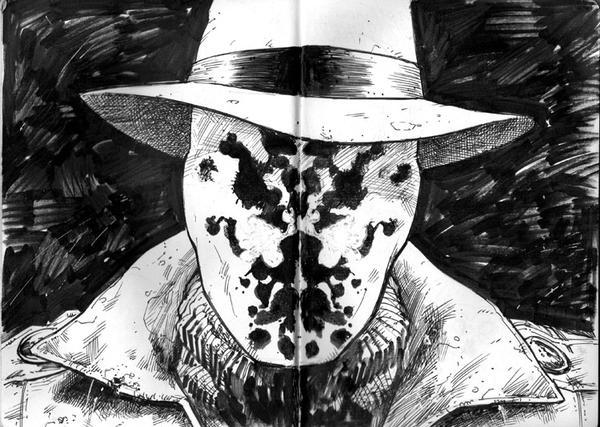
\includegraphics[width=1\textwidth]{images/rorschach.jpg}\\
{\tiny Rorschach}\\ \vspace{.6\textheight}
\end{center}
\end{column}
\end{columns}}


%\frame{
%\frametitle{Optimization Details}
%\begin{itemize}
%\item Optimization Technique
%\begin{itemize}
%\item Genetic Algorithm?
%\item Parameterize space somehow, do non-linear optimization?
%\item Incorporate knowledge that image acquisition is {\em mostly} linear.
%\end{itemize}
%\item Search Space?
%\begin{itemize}
%\item how many training images?
%\item pixels partially turned on, or on/off?  
%\item restrict pixels within an illumination to be connected? convex?
%\item exposure bracketing?  
%\end{itemize}
%\end{itemize}
%}








